\section{Ορισμός μετα-μοντέλου Συνδέσεων}
\label{sec:metamodel_connections}

Το μετα-μοντέλο αυτό περιέχει χαρακτηριστικά που μπορεί να έχει το σύστημα που επιθυμεί ο χρήστης να κατασκευάσει όσον αφορά στη συνδεσμολογία μεταξύ των συσκευών αλλά και στη σύνδεσή τους σε έναν broker. Στο \autoref{fig:metamodel_connections} μπορούμε να δούμε μία απεικόνισή του.

\begin{figure}[!ht]
	\centering
	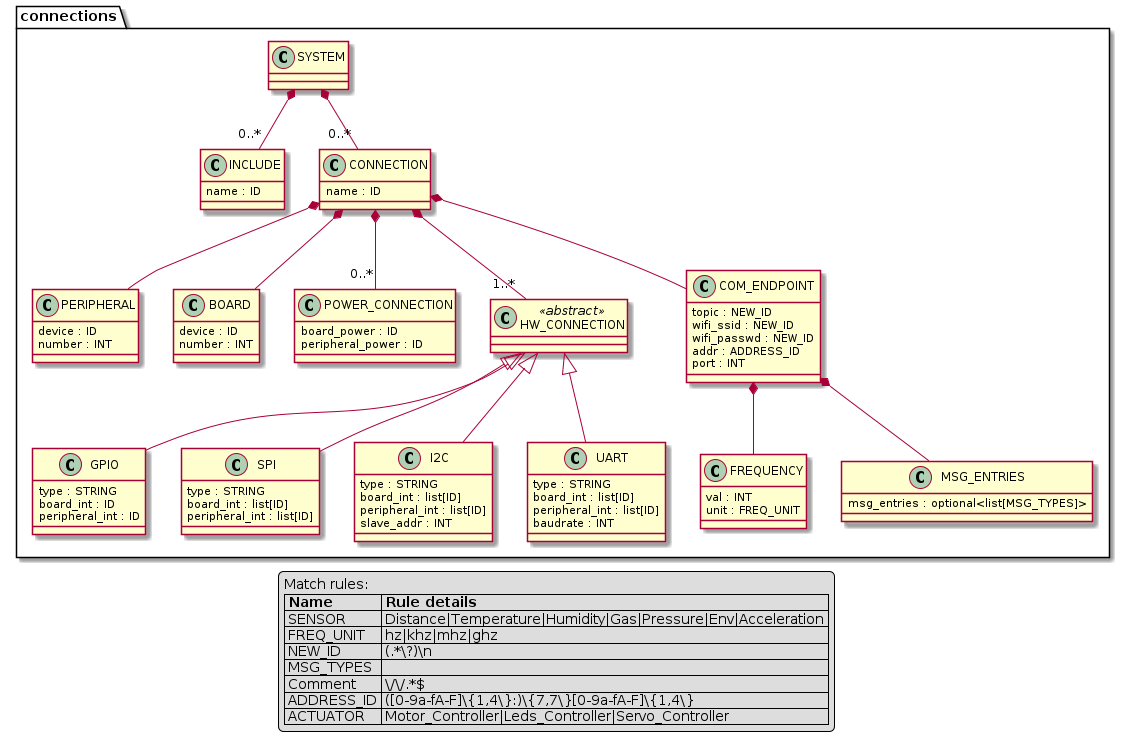
\includegraphics[width=1.0\textwidth]{./images/chapter5/metamodel_connections.png}
	\caption{Μετα-μοντέλο συνδέσεων}
	\label{fig:metamodel_connections}
\end{figure}

\subsection{SYSTEM}
\label{subsec:system}

\subsubsection*{Σύνοψη}

\noindent Το στοιχείο αυτό αναπαριστά ένα σύστημα, το οποίο αποτελείται από συνδέσεις μεταξύ συσκευών (μικροελεγκτές και περιφερειακά).

\subsubsection*{Ιδιότητες και Συσχετίσεις}

\begin{table}[H]
	\begin{center}
		\begin{tabular}{ | c | c | c| m{5.5cm} | }
			\hline
			\rowcolor{Gray}
			\multicolumn{4}{|c|}{\textbf{Συσχετίσεις}}\\
			\hline
			\rowcolor{Gray}
			Όνομα & Τύπος & Πολλαπλότητα & Περιγραφή \\
			\hline
			INCLUDE & Composition-Σύνθεση & 0..* &  Τα ονόματα των συσκευών που απαρτίζουν το σύστημα \\
			\hline
			CONNECTION & Composition-Σύνθεση & 0..* &  Οι συνδέσεις μεταξύ των συσκευών \\
			\hline
		\end{tabular}
		\caption{Συσχετίσεις του \textit{SYSTEM}.}
		\label{tab:system}
	\end{center}
\end{table}

\noindent Δεν περιλαμβάνει περαιτέρω ιδιότητες.

\subsubsection*{Περιορισμοί}

\noindent Δεν υπάρχουν περιορισμοί.

\subsection{INCLUDE}
\label{subsec:include}

\subsubsection*{Σύνοψη}

\noindent Το στοιχείο αυτό είναι το όνομα μιας συσκευής η οποία είναι μέρος του συστήματος, ώστε να ξέρουμε την ύπαρξή της.

\subsubsection*{Ιδιότητες και Συσχετίσεις}

\begin{table}[H]
	\begin{center}
		\begin{tabular}{ | c | c | c| m{5.5cm} | }
			\hline
			\rowcolor{Gray}
			\multicolumn{4}{|c|}{\textbf{Ιδιότητες}}\\
			\hline
			\rowcolor{Gray}
			Όνομα & Τύπος & Πολλαπλότητα & Περιγραφή \\
			\hline
			name & ID & 1..1 &  Το όνομα της συσκευής \\
			\hline
		\end{tabular}
		\caption{Ιδιότητες του \textit{INCLUDE}.}
		\label{tab:include}
	\end{center}
\end{table}

\noindent Δεν περιλαμβάνει περαιτέρω συσχετίσεις.

\subsubsection*{Περιορισμοί}

\noindent Το ID πρέπει να είναι το όνομα συσκευής για την οποία υπάρχει configuration file (.hwd), και άρα να υποστηρίζεται από την παρούσα εργασία.

\subsection{CONNECTION}
\label{subsec:connection}

\subsubsection*{Σύνοψη}

\noindent Το στοιχείο αυτό αναπαριστά τη σύνδεση ενός μικροελεγκτή με ένα περιφερειακό.

\subsubsection*{Ιδιότητες και Συσχετίσεις}

\begin{table}[H]
	\begin{center}
		\begin{tabular}{ | c | c | c| m{5.5cm} | }
			\hline
			\rowcolor{Gray}
			\multicolumn{4}{|c|}{\textbf{Ιδιότητες}}\\
			\hline
			\rowcolor{Gray}
			Όνομα & Τύπος & Πολλαπλότητα & Περιγραφή \\
			\hline
			name & ID & 1..1 &  Το όνομα που θα δοθεί στη σύνδεση \\
			\hline
			\rowcolor{Gray}
			\multicolumn{4}{|c|}{\textbf{Συσχετίσεις}}\\
			\hline
			\rowcolor{Gray}
			Όνομα & Τύπος & Πολλαπλότητα & Περιγραφή \\
			\hline
			PERIPHERAL & Composition-Σύνθεση & 1..1 &  Το περιφερειακό της συγκεκριμένης σύνδεσης \\
			\hline
			BOARD & Composition-Σύνθεση & 1..1 &  Ο μικροελεγκτής της συγκεκριμένης σύνδεσης \\
			\hline
			\scriptsize{POWER\_CONNECTION} & Composition-Σύνθεση & 0..* &  Οι ακροδέκτες που χρησιμοποιούνται για την τροφοδοσία \\
			\hline
			\footnotesize{HW\_CONNECTION} & Composition-Σύνθεση & 1..* &  Οι ακροδέκτες που χρησιμοποιούνται για τη σύνδεση μεταξύ των διεπαφών υλικού \\
			\hline
			\small{COM\_ENDPOINT} & Composition-Σύνθεση & 0..1 &  Τα χαρακτηριστικά σύνδεσης σε κάποιον broker \\
			\hline
		\end{tabular}
		\caption{Ιδιότητες και Συσχετίσεις του \textit{CONNECTION}.}
		\label{tab:connection}
	\end{center}
\end{table}

\subsubsection*{Περιορισμοί}

\noindent Δεν υπάρχουν περιορισμοί.

\subsection{PERIPHERAL}
\label{subsec:peripheral_con}

\subsubsection*{Σύνοψη}

\noindent Το στοιχείο αυτό περιγράφει το περιφερειακό που χρησιμοποιείται σε μία σύνδεση.

\subsubsection*{Ιδιότητες και Συσχετίσεις}

\begin{table}[H]
	\begin{center}
		\begin{tabular}{ | c | c | c| m{5.5cm} | }
			\hline
			\rowcolor{Gray}
			\multicolumn{4}{|c|}{\textbf{Ιδιότητες}}\\
			\hline
			\rowcolor{Gray}
			Όνομα & Τύπος & Πολλαπλότητα & Περιγραφή \\
			\hline
			device & ID & 1..1 & Το όνομα του περιφερειακού \\
			\hline
		    number & INT & 0..1 & Ο αριθμός του περιφερειακού σε περίπτωση που χρησιμοποιείται το ίδιο μοντέλο πολλαπλές φορές στο συγκεκριμένο σύστημα \\
			\hline
		\end{tabular}
		\caption{Ιδιότητες του \textit{PERIPHERAL}.}
		\label{tab:peripheral_con}
	\end{center}
\end{table}

\noindent Δεν περιλαμβάνει περαιτέρω συσχετίσεις.

\subsubsection*{Περιορισμοί}

\noindent Δεν υπάρχουν περιορισμοί.

\subsection{BOARD}
\label{subsec:board_con}

\subsubsection*{Σύνοψη}

\noindent Το στοιχείο αυτό περιγράφει τον μικροελεγκτή που χρησιμοποιείται σε μία σύνδεση.

\subsubsection*{Ιδιότητες και Συσχετίσεις}

\begin{table}[H]
	\begin{center}
		\begin{tabular}{ | c | c | c| m{5.5cm} | }
			\hline
			\rowcolor{Gray}
			\multicolumn{4}{|c|}{\textbf{Ιδιότητες}}\\
			\hline
			\rowcolor{Gray}
			Όνομα & Τύπος & Πολλαπλότητα & Περιγραφή \\
			\hline
			device & ID & 1..1 & Το όνομα του μικροελεγκτή \\
			\hline
			number & INT & 0..1 & Ο αριθμός του μικροελεγκτή σε περίπτωση που χρησιμοποιείται το ίδιο μοντέλο πολλαπλές φορές στο συγκεκριμένο σύστημα \\
			\hline
		\end{tabular}
		\caption{Ιδιότητες του \textit{BOARD}.}
		\label{tab:board_con}
	\end{center}
\end{table}

\noindent Δεν περιλαμβάνει περαιτέρω συσχετίσεις.

\subsubsection*{Περιορισμοί}

\noindent Δεν υπάρχουν περιορισμοί.

\subsection{POWER\_CONNECTION}
\label{subsec:power_connection}

\subsubsection*{Σύνοψη}

\noindent Το στοιχείο αυτό περιγράφει τη σύνδεση (ακροδέκτες) τροφοδοσίας των περιφερειακών από τους μικροελεγκτές.

\subsubsection*{Ιδιότητες και Συσχετίσεις}

\begin{table}[H]
	\begin{center}
		\begin{tabular}{ | c | c | c| m{5.5cm} | }
			\hline
			\rowcolor{Gray}
			\multicolumn{4}{|c|}{\textbf{Ιδιότητες}}\\
			\hline
			\rowcolor{Gray}
			Όνομα & Τύπος & Πολλαπλότητα & Περιγραφή \\
			\hline
			board\_power & ID & 1..1 & Ο ακροδέκτης τροφοδοσίας του μικροελεγκτή \\
			\hline
			peripheral\_power & ID & 1..1 & Ο ακροδέκτης τροφοδοσίας του περιφερειακού \\
			\hline
		\end{tabular}
		\caption{Ιδιότητες του \textit{POWER\_CONNECTION}.}
		\label{tab:power_connection}
	\end{center}
\end{table}

\noindent Δεν περιλαμβάνει περαιτέρω συσχετίσεις.

\subsubsection*{Περιορισμοί}

\noindent Δεν υπάρχουν περιορισμοί.

\subsection{COM\_ENDPOINT}
\label{subsec:com_endpoint}

\subsubsection*{Σύνοψη}

\noindent Το στοιχείο αυτό περιγράφει τα χαρακτηριστικά της σύνδεσης μιας συσκευής σε έναν broker.

\subsubsection*{Ιδιότητες και Συσχετίσεις}

\begin{table}[H]
	\begin{center}
		\begin{tabular}{ | c | c | c| m{5.5cm} | }
			\hline
			\rowcolor{Gray}
			\multicolumn{4}{|c|}{\textbf{Ιδιότητες}}\\
			\hline
			\rowcolor{Gray}
			Όνομα & Τύπος & Πολλαπλότητα & Περιγραφή \\
			\hline
			topic & NEW\_ID & 1..1 & Το όνομα του topic στο οποίο θα στο οποίο θα γίνει publish ή subscribe (ανάλογα αν χρησιμοποιείται αισθητήρας ή ενεργοποιητής αντίστοιχα) \\
			\hline
			wifi\_ssid & NEW\_ID & 1..1 & Το όνομα του wifi δικτύου στο οποίο θα συνδεθεί ο μικροελεγκτής \\
			\hline
			wifi\_password & NEW\_ID & 1..1 & Ο κωδικός του wifi δικτύου στο οποίο θα συνδεθεί ο μικροελεγκτής \\
			\hline
			addr & NEW\_ID & 1..1 & Η IPv6 διεύθυνση του broker με τον οποίο θα επικοινωνήσει ο μικροελεγκτής \\
			\hline
			port & NEW\_ID & 1..1 & Η πύλη σύνδεσης του broker \\
			\hline
			\rowcolor{Gray}
			\multicolumn{4}{|c|}{\textbf{Συσχετίσεις}}\\
			\hline
			\rowcolor{Gray}
			Όνομα & Τύπος & Πολλαπλότητα & Περιγραφή \\
			\hline
			MSG\_ENTRIES & Composition-Σύνθεση & 1..1 &  Τα είδη μηνυμάτων που θα διαμοιραστούν κατά τη συγκεκριμένη σύνδεση \\
			\hline
			FREQUENCY & Composition-Σύνθεση & 0..1 &  Η συχνότητα με την οποία θα γίνονται publish τα μηνύματα στον broker \\
			\hline
		\end{tabular}
		\caption{Ιδιότητες και Συσχετίσεις του \textit{COM\_ENDPOINT}.}
		\label{tab:com_endpoint}
	\end{center}
\end{table}

\subsubsection*{Περιορισμοί}

\noindent Τα topic, wifi\_ssid και wifi\_password μπορούν να πάρουν τιμές σαν ID, με επιπλέον επιλογή να περιλαμβάνουν και παύλες. Αυτό επιτυγχάνεται σύμφωνα με το NEW\_ID που είναι μια \textit{κανονική έκφραση} (\textit{regex}).

\noindent Το addr μπορεί να πάρει τιμές σαν μια διεύθυνση \textit{IPv6} (\textit{Internet Protocol version 6}). Αυτό επιτυγχάνεται σύμφωνα με το ADDRESS\_ID που είναι μια \textit{κανονική έκφραση} (\textit{regex}).

\subsection{MSG\_ENTRIES}
\label{subsec:msg_entries}

\subsubsection*{Σύνοψη}

\noindent Το στοιχείο αυτό περιγράφει τα είδη μηνυμάτων που θα διαμοιραστούν σε μια συγκεκριμένη σύνδεση.

\subsubsection*{Ιδιότητες και Συσχετίσεις}

\begin{table}[H]
	\begin{center}
		\begin{tabular}{ | c | c | c| m{5.5cm} | }
			\hline
			\rowcolor{Gray}
			\multicolumn{4}{|c|}{\textbf{Ιδιότητες}}\\
			\hline
			\rowcolor{Gray}
			Όνομα & Τύπος & Πολλαπλότητα & Περιγραφή \\
			\hline
			msg\_entries & MSG\_TYPES (Enum) & 1..* & Τα είδη μηνυμάτων \\
			\hline
		\end{tabular}
		\caption{Ιδιότητες του \textit{MSG\_ENTRIES}.}
		\label{tab:msg_entries}
	\end{center}
\end{table}

\noindent Δεν περιλαμβάνει περαιτέρω συσχετίσεις.

\subsubsection*{Περιορισμοί}

\noindent Επιλογές των ειδών μηνυμάτων που μπορούν να δηλωθούν:

\begin{itemize}
	\item Distance
	\item Temperature
	\item Humidity
	\item Gas
	\item Pressure
	\item Env
	\item Acceleration
	\item Motor\_Controller
	\item Leds\_Controller
	\item Servo\_Controller
\end{itemize}

\subsection{HW\_CONNECTION}
\label{subsec:hw_connection}

\subsubsection*{Σύνοψη}

\noindent Το στοιχείο αυτό είναα η abstract κλάση για την περιγραφή των συνδέσεων των διεπαφών υλικών των συσκευών.

\subsubsection*{Ιδιότητες και Συσχετίσεις}

\noindent Δεν περιλαμβάνει περαιτέρω ιδιότητες και συσχετίσεις.

\subsubsection*{Περιορισμοί}

\noindent Δεν υπάρχουν περιορισμοί.

\subsection{GPIO}
\label{subsec:gpio_con}

\subsubsection*{Σύνοψη}

\noindent Το στοιχείο αυτό περιγράφει τη σύνδεση δύο GPIO διεπαφών.

\subsubsection*{Ιδιότητες και Συσχετίσεις}

\begin{table}[H]
	\begin{center}
		\begin{tabular}{ | c | c | c| m{5.5cm} | }
			\hline
			\rowcolor{Gray}
			\multicolumn{4}{|c|}{\textbf{Ιδιότητες}}\\
			\hline
			\rowcolor{Gray}
			Όνομα & Τύπος & Πολλαπλότητα & Περιγραφή \\
			\hline
			type & STRING & 1..1 & Το είδος διεπαφής (στην προκειμένη περίπτωση gpio) \\
			\hline
			board\_int & ID & 1..1 & Η διεπαφή του μικροελεγκτή \\
			\hline
			peripheral\_int & ID & 1..1 & Η διεπαφή του περιφερειακού \\
			\hline
			\rowcolor{Gray}
			\multicolumn{4}{|c|}{\textbf{Συσχετίσεις}}\\
			\hline
			\rowcolor{Gray}
			Όνομα & Τύπος & Πολλαπλότητα & Περιγραφή \\
			\hline
			\footnotesize{HW\_CONNECTION} & SuperType-Επέκταση & - &  Το στοιχείο GPIO επεκτείνει το στοιχείο HW\_CONNECTION \\
			\hline
		\end{tabular}
		\caption{Ιδιότητες και Συσχετίσεις του \textit{GPIO}.}
		\label{tab:gpio_con}
	\end{center}
\end{table}

\subsubsection*{Περιορισμοί}

\noindent To type θα πρέπει να έχει την τιμή "gpio", αλλιώς θα εμφανιστεί σφάλμα.

\subsection{I2C}
\label{subsec:i2c_con}

\subsubsection*{Σύνοψη}

\noindent Το στοιχείο αυτό περιγράφει τη σύνδεση μέσω πρωτοκόλλου I2C.

\subsubsection*{Ιδιότητες και Συσχετίσεις}

\begin{table}[H]
	\begin{center}
		\begin{tabular}{ | c | c | c| m{5.5cm} | }
			\hline
			\rowcolor{Gray}
			\multicolumn{4}{|c|}{\textbf{Ιδιότητες}}\\
			\hline
			\rowcolor{Gray}
			Όνομα & Τύπος & Πολλαπλότητα & Περιγραφή \\
			\hline
			type & STRING & 1..1 & Το είδος διεπαφής (στην προκειμένη περίπτωση i2c) \\
			\hline
			board\_int & list[ID] & 1..1 & Οι διεπαφές του μικροελεγκτή \\
			\hline
			peripheral\_int & list[ID] & 1..1 & Οι διεπαφές του περιφερειακού \\
			\hline
			slave\_addr & ID & 1..1 & Η διεύθυνση της διεπαφής που λειτουργεί ως slave \\
			\hline
			\rowcolor{Gray}
			\multicolumn{4}{|c|}{\textbf{Συσχετίσεις}}\\
			\hline
			\rowcolor{Gray}
			Όνομα & Τύπος & Πολλαπλότητα & Περιγραφή \\
			\hline
			\footnotesize{HW\_CONNECTION} & SuperType-Επέκταση & - &  Το στοιχείο I2C επεκτείνει το στοιχείο HW\_CONNECTION \\
			\hline
		\end{tabular}
		\caption{Ιδιότητες και Συσχετίσεις του \textit{I2C}.}
		\label{tab:i2c_con}
	\end{center}
\end{table}

\subsubsection*{Περιορισμοί}

\noindent To type θα πρέπει να έχει την τιμή "i2c", αλλιώς θα εμφανιστεί σφάλμα.

\subsection{SPI}
\label{subsec:spi_con}

\subsubsection*{Σύνοψη}

\noindent Το στοιχείο αυτό περιγράφει τη σύνδεση μέσω πρωτοκόλλου SPI.

\subsubsection*{Ιδιότητες και Συσχετίσεις}

\begin{table}[H]
	\begin{center}
		\begin{tabular}{ | c | c | c| m{5.5cm} | }
			\hline
			\rowcolor{Gray}
			\multicolumn{4}{|c|}{\textbf{Ιδιότητες}}\\
			\hline
			\rowcolor{Gray}
			Όνομα & Τύπος & Πολλαπλότητα & Περιγραφή \\
			\hline
			type & STRING & 1..1 & Το είδος διεπαφής (στην προκειμένη περίπτωση spi) \\
			\hline
			board\_int & list[ID] & 1..1 & Οι διεπαφές του μικροελεγκτή \\
			\hline
			peripheral\_int & list[ID] & 1..1 & Οι διεπαφές του περιφερειακού \\
			\hline
			\rowcolor{Gray}
			\multicolumn{4}{|c|}{\textbf{Συσχετίσεις}}\\
			\hline
			\rowcolor{Gray}
			Όνομα & Τύπος & Πολλαπλότητα & Περιγραφή \\
			\hline
			\footnotesize{HW\_CONNECTION} & SuperType-Επέκταση & - &  Το στοιχείο SPI επεκτείνει το στοιχείο HW\_CONNECTION \\
			\hline
		\end{tabular}
		\caption{Ιδιότητες και Συσχετίσεις του \textit{SPI}.}
		\label{tab:spi_con}
	\end{center}
\end{table}

\subsubsection*{Περιορισμοί}

\noindent To type θα πρέπει να έχει την τιμή "spi", αλλιώς θα εμφανιστεί σφάλμα.

\subsection{UART}
\label{subsec:uart_con}

\subsubsection*{Σύνοψη}

\noindent Το στοιχείο αυτό περιγράφει τη σύνδεση μέσω πρωτοκόλλου UART.

\subsubsection*{Ιδιότητες και Συσχετίσεις}

\begin{table}[H]
	\begin{center}
		\begin{tabular}{ | c | c | c| m{5.5cm} | }
			\hline
			\rowcolor{Gray}
			\multicolumn{4}{|c|}{\textbf{Ιδιότητες}}\\
			\hline
			\rowcolor{Gray}
			Όνομα & Τύπος & Πολλαπλότητα & Περιγραφή \\
			\hline
			type & STRING & 1..1 & Το είδος διεπαφής (στην προκειμένη περίπτωση uart) \\
			\hline
			board\_int & list[ID] & 1..1 & Οι διεπαφές του μικροελεγκτή \\
			\hline
			peripheral\_int & list[ID] & 1..1 & Οι διεπαφές του περιφερειακού \\
			\hline
			baudrate & ID & 1..1 & Το baudrate που χρησιμοποιείται \\
			\hline
			\rowcolor{Gray}
			\multicolumn{4}{|c|}{\textbf{Συσχετίσεις}}\\
			\hline
			\rowcolor{Gray}
			Όνομα & Τύπος & Πολλαπλότητα & Περιγραφή \\
			\hline
			\footnotesize{HW\_CONNECTION} & SuperType-Επέκταση & - &  Το στοιχείο UART επεκτείνει το στοιχείο HW\_CONNECTION \\
			\hline
		\end{tabular}
		\caption{Ιδιότητες και Συσχετίσεις του \textit{UART}.}
		\label{tab:uart_con}
	\end{center}
\end{table}

\subsubsection*{Περιορισμοί}

\noindent To type θα πρέπει να έχει την τιμή "uart", αλλιώς θα εμφανιστεί σφάλμα.

\subsection{FREQUENCY}
\label{subsec:frequency}

\subsubsection*{Σύνοψη}

\noindent Το στοιχείο αυτό περιγράφει τη συχνότητα με την οποία θα γίνονται publish τα μηνύματα στον broker.

\subsubsection*{Ιδιότητες και Συσχετίσεις}

\begin{table}[H]
	\begin{center}
		\begin{tabular}{ | c | c | c| m{5.5cm} | }
			\hline
			\rowcolor{Gray}
			\multicolumn{4}{|c|}{\textbf{Ιδιότητες}}\\
			\hline
			\rowcolor{Gray}
			Όνομα & Τύπος & Πολλαπλότητα & Περιγραφή \\
			\hline
			val & INT & 1..1 & Η τιμή της συχνότητας \\
			\hline
			val & FREQ\_UNIT & 1..1 & Η μονάδα μέτρησης της συχνότητας \\
			\hline
		\end{tabular}
		\caption{Ιδιότητες του \textit{FREQUENCY}.}
		\label{tab:frequency}
	\end{center}
\end{table}

\noindent Δεν περιλαμβάνει περαιτέρω συσχετίσεις.

\subsubsection*{Περιορισμοί}

\noindent Επιλογές των υποστηριζόμενων μονάδων μέτρησης για το max\_freq:

\begin{itemize}
	\item hz
	\item khz
	\item ghz
	\item mhz
\end{itemize}